\documentclass[12pt]{article}
% Required Packages
\usepackage[utf8]{inputenc}
\usepackage{geometry}
\geometry{letterpaper, margin=1in}
\usepackage{subcaption}
\usepackage{amsmath}
\usepackage{graphicx}
\usepackage{booktabs}
\usepackage[numbers,super]{natbib} % For ACS citation style baseline
\usepackage{hyperref}
\usepackage{fontawesome5} % for using icons
\usepackage[dvipsnames]{xcolor}
\usepackage{textcomp}
\usepackage{pdfpages}

\begin{document}

\begin{center}
    \Large \textbf{Lab \#3: Magnetic Susceptibility}
\end{center}
\vspace{0.5em}
\noindent
\begin{minipage}[t]{0.5\textwidth}
    \small
    \textbf{Name:} Yuchen Shi \\
    \textbf{Lab Partner:} Yizhe Dai, Siqi Li \\ 
    \textbf{Section:} 001
\end{minipage}%
\begin{minipage}[t]{0.5\textwidth}
    \small \raggedleft
    \textbf{Date Performed:} 2026-03-03 \\ 
    \textbf{Date Submitted:} 2026-03-24 
\end{minipage}
\vspace{1.5em}


\begin{abstract}
\noindent
In this experiment, the magnetic susceptibilities of NiCl$_2\cdot$6H$_2$O and FeCl$_3\cdot$6H$_2$O solution were measured with an MSB-Auto magnetic susceptibility balance. The volume, mass, and density of the solution were measured indirectly with analytical balance, using water as a volume standard. The measured volume susceptibility was $\chi=0.8790\times10^{-5} V$ for $NiCl_2\cdot 6H_2O$ and $\chi=2.4580\times10^{-5}V$ for $FeCl_3\cdot6H_2O$.
With further calculations, molar susceptibilities were calculated to be $(4.6107 \pm 0.0288)\times10^{-3}$ cm$^3$ mol$^{-1}$ with an error rate of $8.7429\%$ for $NiCl_2\cdot 6H_2O$, and $(1.5870 \pm 0.0126)\times10^{-2}$ cm$^3$ mol$^{-1}$ with an error rate of $4.0656\%$ for $FeCl_3\cdot6H_2O$, in comparison with the literature values. 
The corresponding magnetic moments of $NiCl_2\cdot 6H_2O$ and $FeCl_3\cdot6H_2O$ were $\mu=3.3094 \pm 0.0104 \mu_B$ with an error rate of $4.2823\%$ and $\mu=6.1397 \pm 0.0244 \mu_B$ with an error rate of $2.0121\%$, respectively. The unpaired electrons $n$ were determined to be $2.4572 \pm 0.0100$ with an error rate of $5.5770\%$ for $NiCl_2\cdot 6H_2O$ and $5.2206 \pm 0.0240$ with an error rate of $2.3426\%$ for $FeCl_3\cdot6H_2O$.
Overall, both trails agreed well with the literature values, while the Fe(III) result agreed better with literature than the Ni(II) result. The dominant source of errors was likely to be systematic, including filling to the reference mark, instrument reading uncertainty, and small errors in solution composition.
\end{abstract}


\section*{Introduction}
Magnetic susceptibility is a useful probe of electronic structure. It reflects how a substance responds to an external magnetic field. Compounds with all electrons paired are diamagnetic and are weakly repelled by a magnetic field; while compounds with one or more unpaired electrons are paramagnetic and are attracted to a magnetic field. As a result, for transition-metal compounds, magnetic susceptibility is directly related to the number of unpaired electrons and can provide information about the oxidation state, spin state, etc. In some cases, the observed magnetic moment deviates from a simple spin-only description.\cite{lab_manual}

The purpose of this experiment was to determine the magnetic susceptibilities of \(\mathrm{NiCl_2\cdot 6H_2O}\) and \(\mathrm{FeCl_3\cdot 6H_2O}\) solution using the MSB-Auto magnetic susceptibility balance and analytical weight balance, and then to use additional calculations to estimate the effective magnetic moments and numbers of unpaired electrons for the corresponding metal ions in solution. In this experiment, the instrument measured the volume susceptibility of each solution. So, the density of each solution was determined first from repeated mass measurements of the empty sample tube, the tube filled with water, and the tube filled with the solution to the same reference mark. The known density of water at the measured temperature was then used to determine the calibrated tube volume, which allowed the solution density to be calculated. From this density, the measured volume susceptibility could be converted to the mass susceptibility \(\chi_w\) of the solution, which is further used to calculate the molar susceptibility of the dissolved salt, \(\chi_m\). The conversion was done by correcting for the solvent contribution and accounting for the known mass fraction \(x\) of solute in the prepared solution with the equation from manual \cite{lab_manual}:
\[
\chi_w=\frac{\chi_m}{M}x-0.720(1-x)\times10^{-6}
\]
where \(M\) is the molar mass of the solute and the final term accounts for the diamagnetic contribution of water. Rearrangement of this expression gives the molar susceptibility of the solute, which can then be compared with literature values.

The molar susceptibility can also be used to estimate the effective magnetic moment. In this experiment, the molar susceptibility obtained was converted to SI units with a constant $4\pi\cdot10^{-6}$ before substitution into \cite{lab_manual}
\[
\mu_m = 797.7\mu_B\sqrt{T\chi_m}
\]
where \(T\) is the absolute temperature and \(\mu_m\) is reported in Bohr unit. The magnetic moment can then be used to calculate the approximate number of unpaired electrons through the spin-only expression
\[
\mu_s=\mu_B\sqrt{n(n+2)}
\]
which provides a convenient way to compare the measured magnetic behavior with the expected electronic structures of \(\mathrm{Ni^{2+}}\) and \(\mathrm{Fe^{3+}}\). 

For the present system, \(\mathrm{Ni^{2+}}\) and \(\mathrm{Fe^{3+}}\) are both expected to be paramagnetic, but to different extents. A nickel(II) ion typically has fewer unpaired electrons than a high-spin iron(III) ion, so the iron solution should exhibit the larger magnetic susceptibility and magnetic moment. 

In general, the experiment is expected to provide not only a quantitative measurement of susceptibility, but also a test of whether the observed magnetic properties were consistent with the expected electronic structures of the two metal ions in aqueous solution.


\section*{Experimental}
The empty sample tube was first weighed three times in the same 50 mL beaker on an analytical balance. Deionized water was then added to the tube up to the reference mark near the top, and the filled tube was weighed three times with the same equipment setup. The room temperature was measured by a thermometer to determine the density of the water from a reference table. The water was then removed, and the tube was dried before each solution measurement. Each solution was added in the tube up to the same reference mark, which is used throughout the experiment so that the calibrated volume remained fixed, and the mass was measured for three times same as before.

The MSB-Auto magnetic susceptibility balance was auto-zeroed before measurement. The empty tube was inserted and tared so that the diamagnetic contribution of the glass tube was removed from later readings. The tube plus solution was weighed three times, and the tube was inserted into the balance to measure the volume susceptibility. The mass and magnetic susceptibility data were used for quantity calculations and error propagation analysis.

\section*{Results}
The volume susceptibilities were measured to be $0.8790\times10^{-5}$ for NiCl$_2\cdot$6H$_2$O and $2.4580\times10^{-5}$ for FeCl$_3\cdot$6H$_2$O. The room temperature was measured to be 23.9 $^{\circ}$C and the corresponding water density at was taken as 0.9973240 g cm$^{-3}$ from literature.\cite{kienitz1981litwater} Repeated weight measurements of the empty tube and the tube filled with water were used to determine the calibrated sample volume. Repeated weight measurements of the tube containing each solution then gave the apparent solution masses and densities. All uncertainties were propagated from the repeated mass measurements from the calculations for the mean, standard deviation, and 95\% confidence error.\

Table~\ref{tab:raw} summarizes the raw mass data and the corresponding mean values used in the calculations, and Table~\ref{tab:results} reported the measured and calculated magnetic quantities for the two solutions. The manual calculation process is reported in the Appendix.

\begin{table}[htbp]
    \centering
    \caption{Mass measurements used in the susceptibility calculations.}
    \label{tab:raw}
    \begin{tabular}{p{2.8in}cc}
        \toprule
        Quantity & Individual measurements (g) & Mean $\pm$ uncertainty (g)\\
        \midrule
        Empty tube, $m_E$ & 1.0360, 1.0330, 1.0344 & $1.0345 \pm 0.0037$ \\
        Tube + water, $m_W$ & 1.8490, 1.8509, 1.8502 & $1.8500 \pm 0.0024$ \\
        Tube + NiCl$_2\cdot$6H$_2$O solution, $m_{\mathrm{Ni}}$ & 2.0459, 2.0465, 2.0457 & $2.0460 \pm 0.0010$ \\
        Tube + FeCl$_3\cdot$6H$_2$O solution, $m_{\mathrm{Fe}}$ & 2.0279, 2.0290, 2.0316 & $2.0295 \pm 0.0047$ \\
        \bottomrule
    \end{tabular}
\end{table}

Using formulas from manual \cite{lab_manual} and the guideline, the magnetic quantities were calculated correspondingly. The literature values of $\mu_B$ and n were not directly reported in the literature, instead, they were calculated from literature $\chi_m$ values where details are shown in the Appendix.\cite{miller1985litmag,masson1957litmag}

\begin{table}[htbp]
    \centering
    \caption{Measured and calculated magnetic quantities for the two aqueous salt solutions. The error rate is calculated with the measured molar susceptibility and the literature value. \cite{miller1985litmag,masson1957litmag}}
    \label{tab:results}
    \begin{tabular}{p{2.35in}cc}
        \toprule
        Quantity & NiCl$_2\cdot$6H$_2$O & FeCl$_3\cdot$6H$_2$O \\
        \midrule
        Apparent solution mass, $\Delta m$ (g) & $1.0116 \pm 0.0039$ & $0.9950 \pm 0.0060$ \\
        Density, $\rho$ (g cm$^{-3}$) & $1.2370 \pm 0.0082$ & $1.2168 \pm 0.0099$ \\
        Volume susceptibility, $\chi$ & $0.8790\times10^{-5}$ & $2.4580\times10^{-5}$ \\
        Mass susceptibility, $\chi_w$ (cm$^3$ g$^{-1}$) & $(7.1059 \pm 0.0471)\times10^{-6}$ & $(2.0201 \pm 0.0164)\times10^{-5}$ \\
        Molar susceptibility, $\chi_m$ (cm$^3$ mol$^{-1}$) & $(4.6107 \pm 0.0288)\times10^{-3}$ & $(1.5870 \pm 0.0126)\times10^{-2}$ \\
        Magnetic moment, $\mu_m$ ($\mu_B$) & $3.3094 \pm 0.0104$ & $6.1397 \pm 0.0244$ \\
        Unpaired electrons, $n$ & $2.4572 \pm 0.0100$ & $5.2206 \pm 0.0240$ \\
        Literature $\chi_m$ \cite{miller1985litmag,masson1957litmag} (cm$^3$ mol$^{-1}$) & $4240\times10^{-6}$ & $15250\times10^{-6}$ \\
        Literature $\mu_m$ \cite{miller1985litmag,masson1957litmag} ($\mu_B$) & 3.1735 & 6.0186 \\
        Literature $n$ \cite{miller1985litmag,masson1957litmag}  & 2.3274 & 5.1011 \\
        Error Rate of $\chi_m$& $8.7429\%$ & $4.0656\%$ \\
        Error Rate of $\mu_m$& $4.2823\%$ & $2.0121\%$ \\
        Error Rate of $n$& $5.5770\%$ & $2.3426\%$ \\
        \bottomrule
    \end{tabular}
\end{table}

The apparent mass of water was calculated from $\Delta m_W = m-m_E$, giving
\begin{equation}
\Delta m_W=(0.8156\pm0.0044)\ \mathrm{g}
\end{equation}
and the tube volume was therefore
\begin{equation}
V=\frac{\Delta m_W}{\rho_W}=(0.8178\pm0.0044)\ \mathrm{cm^3}.
\end{equation}
This calibrated volume was assumed to be the same for both solution density calculations.

As summarized in Table~\ref{tab:results}, for NiCl$_2\cdot$6H$_2$O, the measured susceptibility is $0.8790\times10^{-5}V$ and the molar susceptibility is $\chi_m=(4.6107 \pm 0.0288)\times10^{-3}$ cm$^3$ mol$^{-1}$ with an error rate of $8.7429\%$. Further calculations lead to a magnetic moment of $3.3094 \pm 0.0104$ $\mu_B$ with an error rate of $4.2823\%$ and $2.4572 \pm 0.0100$ unpaired electrons with an error rate of $5.5770\%$, larger than the simple spin-only value expected for two unpaired electrons in Ni(II). 

For FeCl$_3\cdot$6H$_2$O, the measured susceptibility is $2.4580\times10^{-5}V$ and the molar susceptibility is $\chi_m=(1.5870 \pm 0.0126)\times10^{-2}$ cm$^3$ mol$^{-1}$ with an error rate of $4.0656\%$. Further calculations lead to a magnetic moment of $6.1397 \pm 0.0244$ $\mu_B$ with an error rate of $2.0121\%$ and $5.2206 \pm 0.0240$ unpaired electrons with an error rate of $2.3426\%$, well matched with the value expected for a high-spin Fe(III) center with five unpaired electrons.

\section*{Discussion}
The transition metals studied were \(\mathrm{Ni^{2+}}\) in \(\mathrm{NiCl_2\cdot 6H_2O}\) and \(\mathrm{Fe^{3+}}\) in \(\mathrm{FeCl_3\cdot 6H_2O}\). As shown in the Figure~\ref{fig:placeholder}, in aqueous solution, they are respectively treated as \([\mathrm{Ni(H_2O)_6}]^{2+}\) and \([\mathrm{Fe(H_2O)_6}]^{3+}\). For \(\mathrm{Ni^{2+}}\), the electron configuration is \(3d^8\). In an octahedral crystal field, it gives $t_{2g}^6e_g^2$ with two unpaired electrons. For \(\mathrm{Fe^{3+}}\), the electron configuration is \(3d^5\). Because \(\mathrm{H_2O}\) is a weak-field ligand, the octahedral complex is expected to be high spin, giving $t_{2g}^3e_g^2$ with five unpaired electrons.

\begin{figure}[htbp]
    \centering
    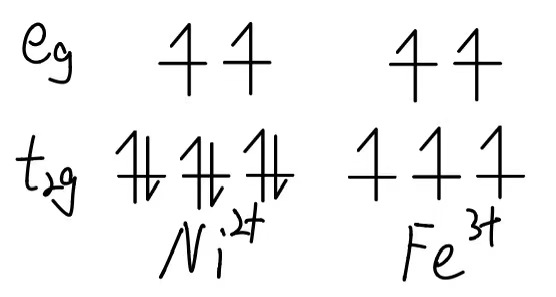
\includegraphics[width=0.5\linewidth]{diagram.jpg}
    \caption{Orbital diagram for each of the transition metals in each for the compounds studied.}
    \label{fig:placeholder}
\end{figure}

The experimental results showed that both \(\mathrm{NiCl_2\cdot 6H_2O}\) and \(\mathrm{FeCl_3\cdot 6H_2O}\) solutions were clearly paramagnetic, as expected for solutions containing \(\mathrm{Ni^{2+}}\) and \(\mathrm{Fe^{3+}}\). The experimental molar susceptibilities were
\[
\chi_{m,\mathrm{Ni}}=(4.6107 \pm 0.0288)\times10^{-3}\ \mathrm{cm^3\,mol^{-1}}
\]
and
\[
\chi_{m,\mathrm{Fe}}=(1.5870 \pm 0.0126)\times10^{-2}\ \mathrm{cm^3\,mol^{-1}}.
\]
Both values were positive, consistent with paramagnetic behavior, and the iron(III) solution showed a larger susceptibility, indicating a stronger response to the applied magnetic field. The difference is chemically reasonable, since \(\mathrm{Fe^{3+}}\) is expected to have more unpaired electrons than \(\mathrm{Ni^{2+}}\), and therefore a larger magnetic moment and larger molar susceptibility.

Comparison with the given literature values \cite{miller1985litmag,masson1957litmag} showed that the experimental value for \(\mathrm{NiCl_2\cdot 6H_2O}\) was higher than the literature value of \(4240\times10^{-6}\ \mathrm{cm^3\,mol^{-1}}\) by \(8.7429\%\), while the experimental value for \(\mathrm{FeCl_3\cdot 6H_2O}\) was higher than the literature value of \(15250\times10^{-6}\ \mathrm{cm^3\,mol^{-1}}\) by \(4.0656\%\). These deviations are not negligible, but they are still small enough that the measured values remain in reasonable agreement with literature. The source of error seems to be systematic, including filling to the reference mark, instrument
reading uncertainty, and small errors in solution composition, which can hardly be resolved with current equipment setup.

The calculated effective magnetic moments were
\[
\mu_{m,\mathrm{Ni}}=(3.3094 \pm 0.0104)\ \mu_B
\]
and
\[
\mu_{m,\mathrm{Fe}}=(6.1397 \pm 0.0244)\ \mu_B.
\]
The corresponding estimated numbers of unpaired electrons were
\[
n_{\mathrm{Ni}}=2.4572 \pm 0.0100
\]
and
\[
n_{\mathrm{Fe}}=5.2206 \pm 0.0240.
\]
These values are also chemically reasonable. A simple spin-only picture would suggest approximately two unpaired electrons for \(\mathrm{Ni^{2+}}\) and five unpaired electrons for high-spin \(\mathrm{Fe^{3+}}\). The value obtained for the iron(III) solution is very close to this expectation, which supports the assignment of a strongly paramagnetic high-spin iron(III) system. The nickel(II) result is also consistent with a paramagnetic ion having about two unpaired electrons, although the measured magnetic moment is slightly higher than the simple spin-only value. 

Several systematic error sources could have affected the results. First, the sample tube had to be filled to the same reference mark each time, both for water and for each solution. Even a very small difference in filling height would change the apparent mass of liquid and therefore the calculated calibrated volume, which would then affect the calculated density and all later quantities derived from it. As we manually added the solution without a precise consistency, the error could be noticeable.

Second, the calculation of molar susceptibility required the known solute mass fractions \(x=0.389\) for \(\mathrm{NiCl_2\cdot 6H_2O}\) and \(x=0.352\) for \(\mathrm{FeCl_3\cdot 6H_2O}\), with a correction for the diamagnetic contribution of water. Any small deviation between the actual prepared concentration and the stated mass fraction would shift the final \(\chi_m\) value.

Another possible source of error was the physical handling of the sample tube. The operating instructions stress elimination of air bubbles, removal of liquid from the outside of the tube, and careful cleaning and drying between measurements. Residual droplets, trapped bubbles, or incomplete drying would change the measured mass and possibly the effective sample volume inside the magnetic field region. 

Moreover, in this experiment, the propagated uncertainties reported do not include an independently measured uncertainty in the susceptibility reading itself, because only a single susceptibility reading was used for each solution. As a result, the reported uncertainties for \(\chi_w\), \(\chi_m\), \(\mu_m\), and \(n\) is the lower-bound uncertainties based mainly on the weighing-derived error propagation. The true total uncertainty in the final results is likely to be larger than the numerical values listed.

Overall, the experiment was successful in measuring the magnetic susceptibility of given solution samples and demonstrating the connection between magnetic susceptibility and electronic structure. The $FeCl_3\cdot 6H_2O$ solution showed a significantly larger molar susceptibility and magnetic moment than the $NiCl_2\cdot 6H_2O$ solution, in agreement with the expectation that \(\mathrm{Fe^{3+}}\) has more unpaired electrons and stronger paramagnetism. Although the experimental values differed from literature values slightly, the deviations were reasonable and can be explained by a combination of instrumental and solution-handling uncertainties. The results therefore support the qualitative and quantitative conclusion that both solutions are paramagnetic, with \(\mathrm{FeCl_3\cdot 6H_2O}\) showing the stronger magnetic response.


\section*{Conclusion}
The magnetic susceptibilities of aqueous \(\mathrm{NiCl_2\cdot 6H_2O}\) and \(\mathrm{FeCl_3\cdot 6H_2O}\) were measured using the MSB-Auto magnetic susceptibility balance. From the measured volume susceptibilities and solution densities, the mass susceptibilities, molar susceptibilities, effective magnetic moments, and estimated numbers of unpaired electrons were obtained through calculations. The experimental molar susceptibilities were \((4.6107 \pm 0.0288)\times10^{-3}\ \mathrm{cm^3\,mol^{-1}}\) for \(\mathrm{NiCl_2\cdot 6H_2O}\) and \((1.5870 \pm 0.0126)\times10^{-2}\ \mathrm{cm^3\,mol^{-1}}\) for \(\mathrm{FeCl_3\cdot 6H_2O}\), corresponding to percent deviations of \(8.7429\%\) and \(4.0656\%\) from literature values, respectively. 

Overall, the results were in reasonable agreement with literature and were consistent with the expected paramagnetic behavior of \(\mathrm{Ni^{2+}}\) and \(\mathrm{Fe^{3+}}\). The remaining discrepancies were most likely caused by systematic effects, such as slight differences in filling to the reference mark, uncertainty in the MSB measurements, and solution-handling error.


\newpage
% References section 
% Must follow American Chemical Society (ACS) format. 
\bibliographystyle{achemso} % Uses the ACS formatting style
\bibliography{references} % Ensure you create a references.bib file in your directory

\newpage
\section*{Appendix}
\addcontentsline{toc}{section}{Appendix}
% Include supplementary material (raw output, sample calculations) 
The raw data and corresponding analysis script are available on \href{https://github.com/EasonShi0624/26Spring-PChemLab/tree/main/Lab_3_Magnetic_Susceptibility}{\textcolor{RoyalBlue}{GitHub} \faGithub}

\begin{figure}[htbp]
    \centering
    
\includegraphics[width=0.7\linewidth, keepaspectratio, page=1]{Lab Computation.pdf}
    \caption{Computations of Values and Error Analysis (Page 1)}
    \label{fig:lab_comp_p1}
\end{figure}

\begin{figure}[htbp]
    \centering
    
\includegraphics[width=0.9\linewidth, keepaspectratio, page=2]{Lab Computation.pdf}
    \caption{Computations of Values and Error Analysis (Page 2)}
    \label{fig:lab_comp_p1}
\end{figure}


\begin{figure}[htbp]
    \centering
    
\includegraphics[width=0.9\linewidth, keepaspectratio, page=3]{Lab Computation.pdf}
    \caption{Computations of Values and Error Analysis (Page 3)}
    \label{fig:lab_comp_p1}
\end{figure}


\begin{figure}[htbp]
    \centering
    
\includegraphics[width=0.9\linewidth, keepaspectratio, page=4]{Lab Computation.pdf}
    \caption{Computations of Values and Error Analysis (Page 4)}
    \label{fig:lab_comp_p1}
\end{figure}


\begin{figure}[htbp]
    \centering
    
\includegraphics[width=0.9\linewidth, keepaspectratio, page=5]{Lab Computation.pdf}
    \caption{Computations of Values and Error Analysis (Page 5)}
    \label{fig:lab_comp_p1}
\end{figure}

\begin{figure}[htbp]
    \centering
    
\includegraphics[width=0.9\linewidth, keepaspectratio, page=6]{Lab Computation.pdf}
    \caption{Computations of Values and Error Analysis (Page 6)}
    \label{fig:lab_comp_p1}
\end{figure}


\begin{figure}[htbp]
    \centering
    
\includegraphics[width=0.9\linewidth, keepaspectratio, page=7]{Lab Computation.pdf}
    \caption{Computations of Values and Error Analysis (Page 7)}
    \label{fig:lab_comp_p1}
\end{figure}

\begin{figure}[htbp]
    \centering
    
\includegraphics[width=0.9\linewidth, keepaspectratio, page=8]{Lab Computation.pdf}
    \caption{Computations of Values and Error Analysis (Page 8)}
    \label{fig:lab_comp_p1}
\end{figure}



\begin{figure}[htbp]
    \centering
    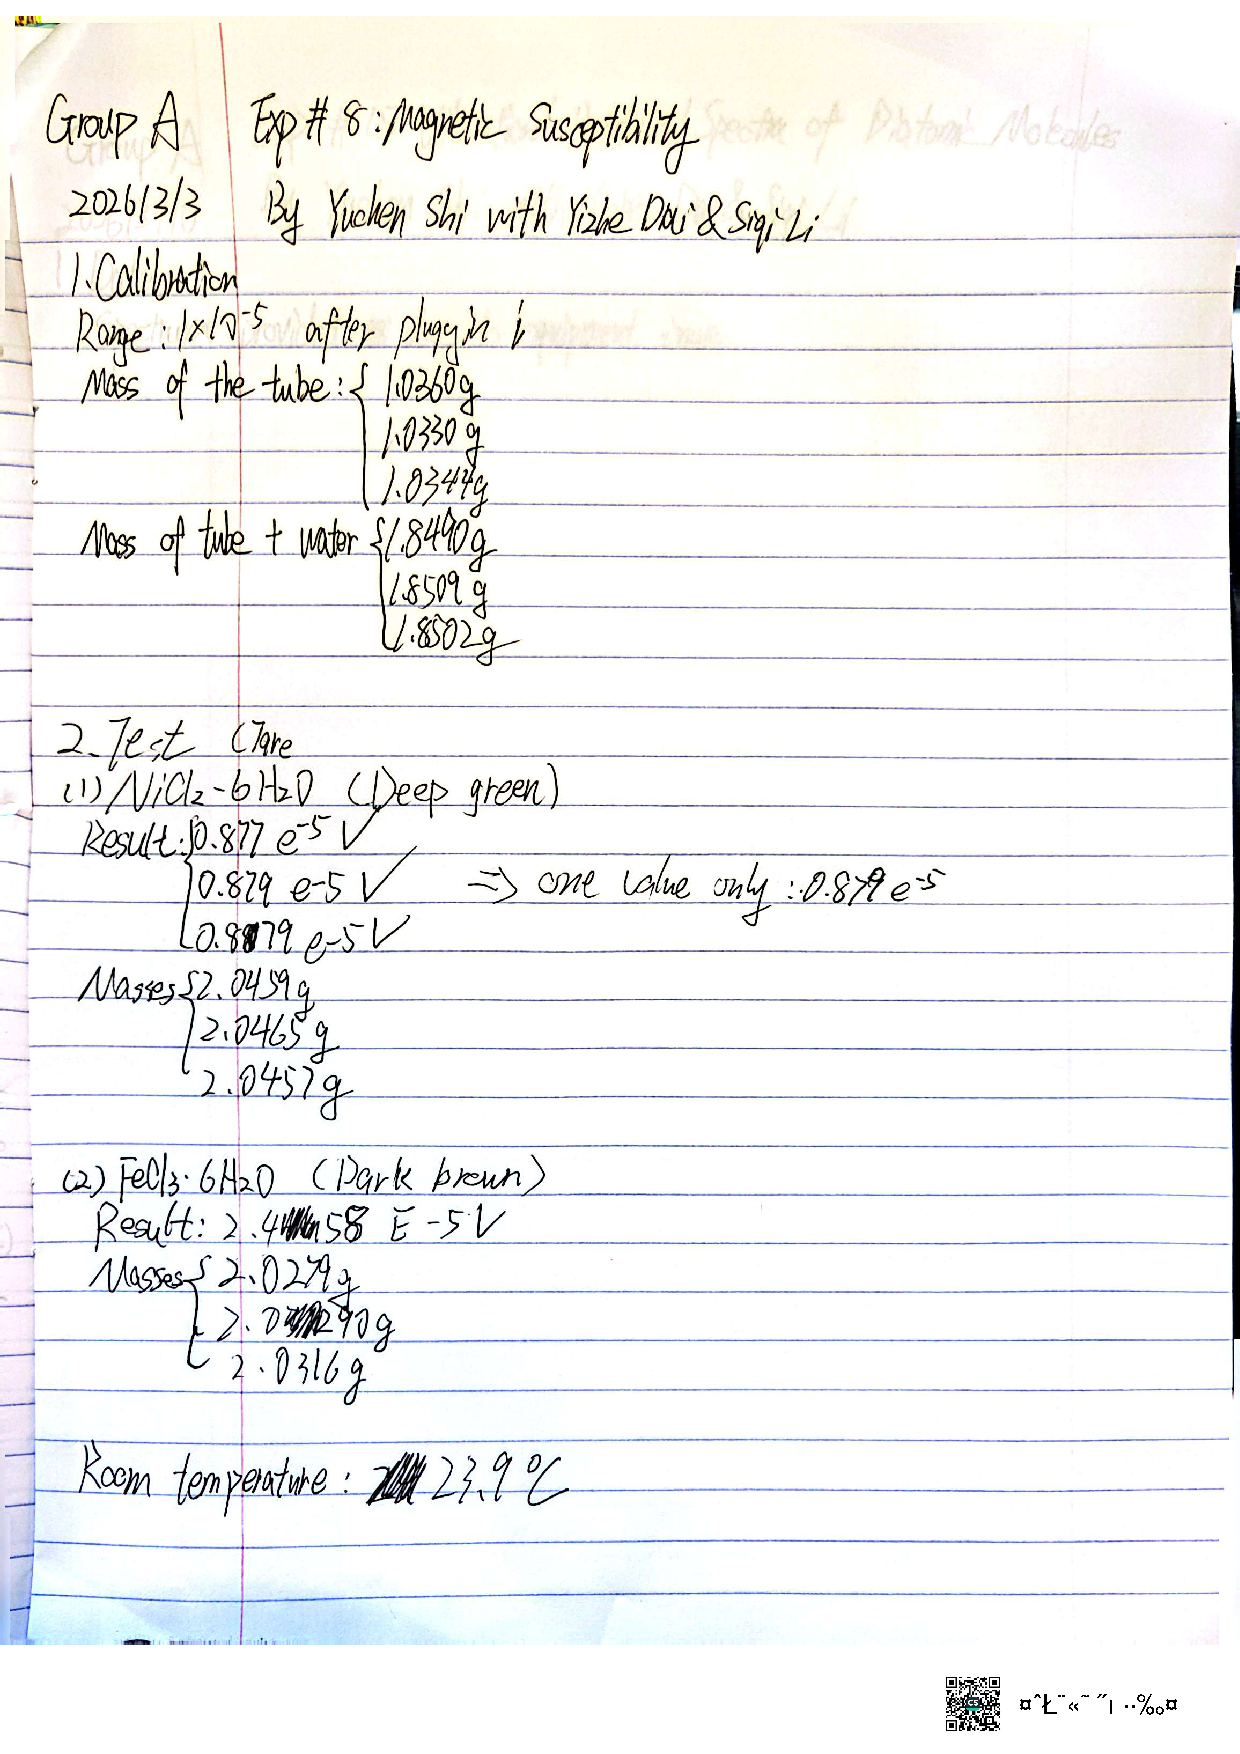
\includegraphics[width=0.9\linewidth, keepaspectratio, page=1]{lab_note.pdf}
    \caption{Raw Lab Notes}
    \label{fig:lab_notes}
\end{figure}


\end{document}